% 基本概念

\subsection{描述一个态}

我们用如下记号: $|\alpha\rangle$ 来描述一个态,这种描述也称为“右矢”. 从某种程度上,它可以理解为我们线性代数里面学过的列矢量:
\begin{equation}
|\alpha\rangle = \left(\begin{matrix}x_1\\x_2\\ \vdots\\ x_n\end{matrix}\right)
\end{equation}

当然,这么写出来的话,肯定要指明我们实在怎样的一组坐标下面来进行这个描述的. 一旦清楚的说明坐标了之后,这个态的意义也就明确了起来. 在量子力学的课程中,一个很容易造成困扰的概念就是“叠加态”. 请大家一定记住,叠加态并不是什么奇怪的事情. 比如,你在三维直角坐标系中,有一个点 $(1, 1, 1)/\sqrt3$,你会觉得“不可思议!竟然可以同时处于 $x$ 轴、 $y$ 轴、 $z$ 轴的混合态” 吗?不会吧. 所以,在量子力学里面,你也不必对此大惊小怪——大家其实是同样的数学结构.

有右矢自然就有左矢. 代数的讲,一个右矢对应的左矢是它的Hermitian共轭\footnote{其实这有约定俗成的翻译:厄米;然而,这个翻译实在是不能达意,我并不打算使用它.},通常会用 $h. c$ 来表示(Hermitian Conjugation). 共轭大家肯定知道,就是复数里面把幅角取反即可了,但是如果在此基础上再做一个转置的话,就构成了Hermitian共轭,形成了左矢,也就是一个行向量.
\begin{equation}
\langle\alpha| = (x_1^*\ x_2^*\ \cdots\ x_n^*)
\end{equation}

举一个简单的例子,

\begin{exam}{}
如果规定
\begin{equation}
|\alpha\rangle = \frac{1}{\sqrt{2}}\left(\begin{matrix}\I \\1\end{matrix}\right) 
\end{equation}
那么
\begin{equation}
\langle\alpha| = \frac{1}{\sqrt{2}}(-\I, 1)
\end{equation}
\end{exam}

左矢和右矢之间可以做内积,就像一个行矢量和列矢量做内积(乘法)一样,得到一个数 $\langle\alpha|\beta\rangle = x \in \mathbb{C}$. 还是刚才那个例子,

\begin{exam}{}
\begin{equation}
\langle\alpha|\alpha\rangle = 1
\end{equation}
\end{exam}

这样一组对应的左矢和右矢内积得 1 的称为单位向量,也叫归一的向量,归一的态,等等很多叫法. 如果一个态没有归一,对它进行归一化的过程为
\begin{equation}
|\beta\rangle\rightarrow\frac{|\beta\rangle}{\sqrt{\langle\beta|\beta\rangle}}
\end{equation}

这里面其实用到了内积的一个小性质: $\langle\alpha|\beta\rangle = (\langle\beta|\alpha\rangle)^*$. 读者可以验证一下.

我们说了这么久的态,但是我们知道在波动力学里面,我们描述一个态是利用它的波函数,一般是坐标的函数 $\psi(x)$. 这个和我们的态有什么关系呢?

其实很有关系的. 我先不着急透露,我们先想想内积的几何意义. $\langle\alpha|\beta\rangle$ 是不是相当于求出 $|\beta\rangle$ 是有多少成分在 $|\alpha\rangle$ 上么?也就是说,
\begin{equation}
|\beta\rangle = \langle\alpha|\beta\rangle|\alpha\rangle + \text{ 与}|\alpha\rangle\text{垂直的成分} 
\end{equation}

那我们考虑这么一组态\footnote{实际上有不可数无穷个态,而且归一的办法和我们之前说的不完全一样,但是这里就先不管数学上这样会不会带来问题了}, $|x\rangle$,它们代表一个态被完全的限制在了 $x$ 处无法移动. 那么,一个归一的态 $|\psi\rangle$ 如果能写成坐标空间的波函数形式的话,其最有可能的样子就是
\begin{equation}
\psi(x) = \langle x|\psi\rangle
\end{equation}

由于无论是波函数还是态矢量(右矢),差一个复数相位都是不会有什么区别的,所以我们的粒子在 $x\rightarrow x'+\Delta x'$ 找到的概率,就像一般的量子力学问题里面说的那样,是
\begin{equation}
\int_{x'}^{x'+\Delta x'}|\psi(x)|^2 \dd{x} = \int_{x'}^{x'+\Delta x'} \langle\psi|x\rangle\langle x|\psi\rangle
\end{equation}

如果对全空间积分,这个概率是 1,也就是说
\begin{equation}
\int_{-\infty}^{\infty}\langle\psi|x\rangle\langle x|\psi\rangle = 1
\end{equation}

这是一个平凡的结论,但是实际上这很有一点深意的,本章中间的部分可以看到.

捎带说一句,像 $\langle x|\alpha\rangle$ 这样,可以叫 $|\alpha \rangle$ 的 $x$ 表象. 类似的还有动量表象等. 不同表象之间的变换等问题随后会讲.

\subsection{算符}

首先介绍一个很重要的算符:单位算符. 别急,这个是很无聊,但是却有很重要的作用. 而且,我们介绍的并不是那么无聊的形式.

考虑一组完备正交归一的态 $|\lambda_i\rangle$. 单位算符 $I$ 就可以写成
\begin{equation}\label{Basics_eq11}
I = \sum_i |\lambda_i\rangle\langle\lambda_i|
\end{equation}

这就被称为 \bb{resolution of identity}. 为了便于理解,我们来举一个例子.

\begin{exam}{}
三维空间一个矢量
\begin{equation}
\bvec{v} = v_x\bvec{i} + v_y\bvec{j} + v_z \bvec{k} 
\end{equation}
其中,$v_x, v_y, v_z$ 可以通过 $\langle i\ (or\ j, k)|v\rangle$ 得到.

也就是说,
\begin{equation}
\begin{split}
|v\rangle &= v_x|i\rangle + v_y|j\rangle + v_z|k\rangle = |i\rangle\langle i|v\rangle + |j\rangle\langle j|v\rangle + |k\rangle\langle k|v\rangle\\ &= (|i\rangle\langle i|+|j\rangle\langle j|+|k\rangle\langle k|)|v\rangle
\end{split}
\end{equation}
\end{exam}{}
正如\autoref{Basics_eq11},我们有
\begin{equation}
|\alpha\rangle = \sum_i |\lambda_i\rangle\langle\lambda_i|\alpha\rangle
\end{equation}

还有很多一般的关于算符的理论. 相信通过前面的理解,我们知道算符在某一组特定的正交完备归一基 $|\lambda_i\rangle$ 下可以表示为矩阵,而矩阵元
\begin{equation}
A_{ij} = \langle\lambda_i|A|\lambda_j\rangle
\end{equation}
一个物理量显然是一个实数,这实际上要求了它对应的算符是 Hermitian 算符,即
\begin{equation}
\hat{A} = \hat{A}\Her,\quad i.e.,\quad A_{ij} = A_{ji}^*
\end{equation}
(实际上,在满足 $\mathcal{PT}$ 对称性下这两件事情并不完全一致,不是Hermitian算符也可以得到全部实数的本征值,在本书中不考虑这种事情)而不是物理量的算符并不非要是Hermitian的,如
\begin{equation}
\left(\begin{matrix}0 & 1\\0 & 0\end{matrix}\right) \quad \& \quad \left(\begin{matrix}0 & 0\\1 & 0\end{matrix}\right)
\end{equation}
介绍几个重要的二维 Hermitian:
\begin{equation}\label{Basics_eq18}
\sigma_0 = \left(\begin{matrix}1 & 0\\0 & 1\end{matrix}\right),
\quad\sigma_1 = \left(\begin{matrix} 0 & 1\\1 & 0\end{matrix}\right),
\quad\sigma_2 = \left(\begin{matrix} 0 & -\I\\ \I & 0\end{matrix}\right),
\quad\sigma_3 = \left(\begin{matrix} 1 & 0\\0 & -1\end{matrix}\right)  
\end{equation}
上面四个矩阵被称为 \bb{Pauli 矩阵},有的时候也会写成四维(矩阵)矢量的形式,$\bvec{\sigma}$.

这四个矩阵十分重要,尤其是在研究自旋 $1/2$ 体系的时候. 这部分内容在后面讲角动量的时候你会时常见到.

关于算符还有很多内容,考虑到这是一个启发性的讲义,这里就不赘述了. 我们可以从Exercise里面逐步学习:

\begin{exer}{}\label{Basics_exe1}
定义
\begin{equation}
\hat{A} = \left(
\begin{matrix}
0 & 0 & 0 & \cdots \\
1 & 0 & 0 & \cdots \\
0 & \sqrt{2} & 0 & \cdots\\
0 & 0 & \sqrt{3} & \cdots\\
  &  &  &  \ddots
\end{matrix}
\right)
\end{equation}
求出下面算符的本征态和对应的本征值:
\begin{equation}
\hat{H} = \hat{A}\Her\hat{A} + \frac{1}{2}
\end{equation}
\end{exer}

接下来我们看一下算符的对易关系,其实与其相关的矩阵的对易关系想必你们都学过:
\begin{equation}
\begin{split}
[\hat{A},\hat{B}] \overset{def}{\equiv}\hat{A}\hat{B} - \hat{B}\hat{A}\\
\{\hat{A},\hat{B}\} \overset{def}{\equiv}\hat{A}\hat{B} + \hat{B}\hat{A}\\
\end{split}
\end{equation}
这里不仅介绍了对易,也介绍了反对易. 这两者同样常见,不同的是,前者经常出现于玻色体系,而后者经常出现于费米体系.

\begin{exer}{}
在\autoref{Basics_exe1} 中,我们定义了算符 $\hat{A}$. 那么,请计算
\begin{equation}
[\hat{A},\hat{A}\Her] = ?
\end{equation}
\end{exer}

\begin{exer}{}
试证明,对于 $\forall \hat{A}, \hat{B}, \hat{C}$
\begin{equation}
[\hat{A},[\hat{B},\hat{C}]] + [\hat{B},[\hat{C},\hat{A}]] + [\hat{C},[\hat{A},\hat{B}]] = 0
\end{equation}
\end{exer}

接下来简要介绍一下算符的完备性,证明暂时略去. 可以证明的是,存在逆的Hermitian算符,即存在 $\hat{B}\hat{A} = I$ 的时候,如果这个Hermitian算符的本征态维数有限,那么这个本征态是完备的. 如果无限维,这件事情不一定成立. 至于有人问为什么无限维会带来bug呢?举个简单的例子证明无限维的时候好多概念都用不了.

\begin{exam}{}
定义\footnote{从这里开始,后面很可能有的时候算符不写它的那个“帽子” $\hat{\ }$ 了.}一个无限维的完备正交归一解为 $|i\rangle, i = 0, 1, \cdots \infty$,那么考虑算符
\begin{equation}
A =  \sum_{i = 0}^{\infty} |i\rangle\langle i+1|,\quad B = \sum_{i = 1}^{\infty}|i\rangle\langle i-1|
\end{equation}
那么,显然有
\begin{equation}
AB = I,\quad BA = I - |0\rangle\langle0|
\end{equation}
也就是说,逆矩阵这件事情实际上在无限维的时候定义有一定困难.
\end{exam}

以上就是关于算符的一些一般性质.

\subsection{特殊的算符}

我们知道,大多数情况下,一个粒子的哈密顿量都会包含动能部分,而动能的表示又是依靠动量的. 很常见的,我们就会考虑动量算符 $\hat p$. 这个算符的本征态和对应的本征值为
\begin{equation}
\hat p|p_0\rangle = p_0 |p_0\rangle
\end{equation}
而由于是连续的谱,归一化条件将是利用delta函数的
\begin{equation}
\langle p_1|p_2\rangle = \delta(p_1-p_2)
\end{equation}

这种连续的谱也会发生在坐标算符 $\hat x$ 上. 类似的有
\begin{align}
\hat x|x_0\rangle &= x_0 |x_0\rangle\\
\langle x_1|x_2\rangle &= \delta(x_1-x_2)
\end{align}

我们前面介绍过的resolution of identity,这里的形式也需要改变:
\begin{gather}
\int \dd{p}|p\rangle\langle p| = I\\
\int \dd{x}|x\rangle\langle x| = I
\end{gather}
不过这些都是小变化,仔细想想的话,其实很容易理解.

我们接下来要考虑的实际上是一个非常奇怪的问题: $\langle p|x\rangle = ?$. 答案很简单,形式为
\begin{equation}
\langle p|x\rangle = \frac{1}{\sqrt{2\pi \hbar}}\E^{-\I px/\hbar}
\end{equation}
但是具体怎么做的呢?我们先看一个貌似与这个问题并不是很相关的问题:平移问题.

让我们考虑沿着 $x$ 方向的平移算符 $\hat{\mathcal J}$: 
\begin{equation}
\hat{\mathcal{J}}(\dd{x'})|x'\rangle = |x'+\dd{x'}\rangle
\end{equation}
有了这组性质之后我们实际上可以得到任何态 $|\alpha\rangle$ 是如何在这样一个平移下变换的,因为我们可以把它展开成坐标本征态的线性组合
\begin{equation}
\hat{\mathcal{J}}(\dd{x'})|\alpha\rangle = \int\hat{\mathcal{J}}(\dd{x'})|x'\rangle\langle x'|\alpha\rangle \dd{x'} = \int|x'+\dd{x'}\rangle\langle x'|\alpha\rangle \dd{x'}
\end{equation}
有几点值得注意:这个算符满足很多性质,比如它是Unitary的,再比如说它是非常常见的可以线性组合的
\begin{equation}
\begin{cases}
\hat{\mathcal{J}}(\dd{x'})\hat{\mathcal{J}}\Her (\dd{x'}) = 1\\
\hat{\mathcal{J}}(\dd{x'})\hat{\mathcal{J}}(\dd{x''}) = \hat{\mathcal{J}}(\dd{x'} + \dd{x''})\\
\hat{\mathcal{J}}(-\dd{x'}) = \hat{\mathcal{J}}^{-1}(\dd{x'})\\
\hat{\mathcal{J}}(0) = I
\end{cases}
\end{equation}
考虑到量子力学的基本假设\footnote{我后面\bb{可能}会总结一下基本假设,但也可能不总结了orz}, $[x,p] = \I\hbar$,我们注意到
\begin{gather}
\hat{x}\hat{\mathcal{J}}(\dd{x'})|x'\rangle = (x'+\dd{x'})|x'+\dd{x'}\rangle\\
\hat{\mathcal{J}}(\dd{x'})\hat{x}|x'\rangle = x'|x'+\dd{x'}\rangle
\end{gather}
也就是说
\begin{equation}
[\hat{x},\hat{\mathcal{J}}(\dd{x'})] \sim \dd{x'}
\end{equation}
这里面的约等于号是考虑到 $|x'+\dd{x'}\rangle \sim |x'\rangle$. 利用在 $\dd{x'}\rightarrow0$ 的时候 $\hat{\mathcal{J}}(\dd{x'})\rightarrow1$,我们得到
\begin{equation}
\hat{\mathcal{J}}(\dd{x'}) \sim 1-\frac{\I}{\hbar}\hat{p}\dd{x'}
\end{equation}

\begin{exam}{}
可以证明 $\hat{P}$ 是Hermitian的. 一般这种问题的做法是看矩阵元,比如我有一套本征态 $|i\rangle$,定义 $P_{ij} \equiv \langle i|P|j\rangle$. 如果他是Hermitian的,那么 $P_{ij} = P_{ji}^*$. 但是这里的话,我们没有办法选取离散的本征态,不过即使只是连续本征态,也是可以的. 最直觉的做法就是选取坐标本征态,我们规定 $P(x,x') = \langle x|P|x'\rangle$. 我们只需要证明 $P(x,x') = P(x',x)^*$. 这里简要地给出一个“令人信服”但不那么严格的说法.

我们有一个最方便的办法来计算,就是利用 $\dd{x'}$ 很小的时候的 $\hat{\mathcal{J}}(\dd{x'})$.
\begin{equation}
\langle x|\hat{\mathcal{J}}(a)|x'\rangle \sim \langle x|x'\rangle - \frac{\I}{\hbar} a \langle x|P|x'\rangle
\end{equation}
也就是说
\begin{equation}
P(x,x') \sim \I\frac{\hbar}{a}[\langle x|\hat{\mathcal{J}}(a)|x'\rangle - \langle x|x'\rangle] = \I\frac{\hbar}{a}[\langle x|x'+a\rangle - \langle x|x'\rangle]
\end{equation}
而很类似的
\begin{gather}
P(x',x) \sim \I\frac{\hbar}{a}[\langle x'|x+a\rangle - \langle x'|x\rangle]\\
P(x,x')^* \sim -\I\frac{\hbar}{a} [\langle x'+a|x\rangle - \langle x'|x\rangle] = \I\frac{\hbar}{a} [\langle x'|x\rangle - \langle x'+a|x\rangle]
\end{gather}
取 $a\rightarrow0$,上面的式子严格等于,而且两者的关系更一目了然.
\end{exam}

\subsection{投影算符}

这是一个概念,看起来并不是很有趣,但是我们在后面学习微扰理论% 链接未完成
的时候会发现它很重要.

它一般指这样一个算符:我们现在有一组正交完备归一的基 $\{|\alpha_i\rangle\}$. 我们很关心一个初始在 $|\alpha_j\rangle$ 的基的行为,并且可以预料到,在其刚刚开始演化的时候,其大部分成分都还这个态上. 这就有点像你把一根直线转了一个小角度,它沿原来方向的分量还是很大,如\autoref{Basics_fig1}.

\begin{figure}[ht]
\centering
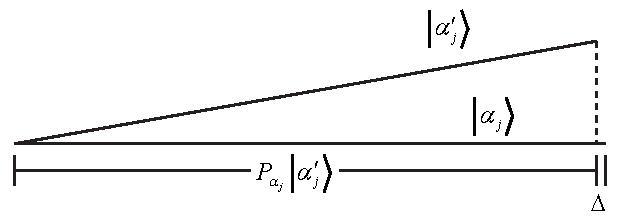
\includegraphics[width=8.7cm]{./figures/Basics1.pdf}
\caption{偏移一点的矢量与投影} \label{Basics_fig1}
\end{figure}

很显然的,这个投影算符就可以用 $|\alpha_j\rangle\langle\alpha_j|$ 来表示. 我们还是利用我们之前介绍过的一个例子来说明.

\begin{exam}{}
三维空间一个矢量
\begin{equation}
\bvec{v} = v_x\bvec{i} + v_y\bvec{j} + v_z \bvec{k}
\end{equation}
如果我要获得它的 $x$ 方向的投影,我首先要保证它在 $x$ 方向上,其次要保证它的大小. 于是,最后得到
\begin{equation}
\bvec{v}_x = v_x\bvec{i} = (\bvec{v}\cdot\bvec{i})\bvec{i} = \langle i|v\rangle |i\rangle = |i\rangle\langle i| \bvec{v}
\end{equation}
\end{exam}

投影算符不仅指投影到一个方向的,还指投影到一个平面上的投影算符,或者投影到Hilbert空间上更“高维度”的空间.

这个投影算符虽然现在看起来没有什么用,但是后面你会看到它的作用的. 几个有趣的性质读者可以作为练习

\begin{exer}{}
请读者证明:如果 $\hat{P}$ 是投影算符,则

(1) $\hat{P}\hat{P} = \hat{P}$

(2) $1-\hat{P}$ 也是投影算符.
\end{exer}

\subsection{算符的函数}

我们很多时候可以写一些算符的函数来简化算符. 大部分时候这种函数都是一目了然的,比如 $\hat{A}^2 = \hat{A}\cdot\hat{A}$,但有的时候也存在一些很微妙的东西. 值得注意的是,无论什么时候,都要记得算符不一定是可对易的.

一个简单的函数,$f(\hat{A}) = \hat{A}^2$ 就容易造成初学者的失误. 比如
\begin{equation}
f(\hat{A}+\hat{B}) = \hat{A}^2 + \hat{A}\hat{B} + \hat{B}\hat{A} + \hat{B}^2
\end{equation}
稍微复杂点的函数,比如
\begin{equation}
\exponential(\hat{A}) = I + \hat{A} + \frac{1}{2!}\hat{A}^2 + \cdots
\end{equation}
也是非常常见的一种算符函数.

\begin{exer}{}
考虑一个体系,它的Hilbert空间是二维的,并且计 $\left(\begin{matrix}1 \\0\end{matrix}\right) = |\!\uparrow\rangle, \left(\begin{matrix}0 \\1\end{matrix}\right) = |\!\downarrow\rangle$. 现在有一个算符
\begin{equation}
\hat{U} = \exp(\I\alpha(t) \sigma_x)
\end{equation}
其中,$\sigma_x$ 是\autoref{Basics_eq18} 定义的 Pauli 矩阵, 那么求
\begin{equation}
\hat{U} \left(\begin{matrix}1 \\0\end{matrix}\right) = ? 
\end{equation}
显然,我们有
\begin{equation}
\hat U= I_{2\times2} + \alpha(t) \sigma_x + \frac{1}{2!}\left(\alpha(t) \sigma_x\right)^2 + \dots
\end{equation}
由于Pauli矩阵有很好的性质:
\begin{equation}
\sigma_x^2 = I_{2\times2}
\end{equation}
我们有
\begin{equation}
\begin{split}\hat U &= \left(1 - \frac{1}{2!}\alpha(t)^2 + \frac{1}{4!}\alpha(t)^4  \cdots\right)  I_{2\times2} + \left(\alpha(t) + \frac{1}{3!}\alpha(t)^3 + \cdots \right)\I \sigma_x\\
& = \cos\alpha(t) I_{2\times2} + \sin\alpha(t) \I\sigma_x 
\end{split}
\end{equation}
从而,我们有
\begin{equation}
\hat U \left(\begin{matrix}1 \\0\end{matrix}\right)  =  \left(\begin{matrix}\cos\alpha(t) \\ \I \sin\alpha(t)\end{matrix}\right)
\end{equation}

这个例子实际上在我们后面看到动力学分析中是一个很常见的``量子演化问题''的基本处理. 以后%未完成:原为 chap3, 然而这章并没有开始写.
我们会再次看到这个问题的.
\end{exer}

以上是一个带答案的练习,现在我们出一个证明性的练习.

\begin{exer}{}
求证:
\begin{equation}
\E^{\hat A}\hat B \E^{-\hat A} = \hat{B} + [\hat A,\hat B] + \frac{1}{2!} [\hat A, [\hat A,\hat B]] + \cdots
\end{equation}
这个等式叫做Baker-Hausdorff formula,我们可能会经常地遇到这个式子.
\end{exer}

\subsection{$^\star$ 密度矩阵,与量子信息基本概念}

量子信息可以说是只要具备完善的量子力学知识就能够入门,但是入的好不好得看初等数学功力的一个方向.

量子信息里面一个重要的概念就是\bb{密度矩阵}. 对于\bb{纯态(Pure State)}, 即一个可以被用态矢量描述的态, 归一态矢量为 $|\psi\rangle$,其密度矩阵可以用
\begin{equation}
\hat\rho_{\psi} = |\psi\rangle\langle\psi|
\end{equation}
来描述. 这样的描述可以略去态矢量的相位,是自由度更小的更“好”的描述.

纯态密度矩阵有很多性质,比如
\begin{equation}
\hat\rho = \hat\rho\Her,\ \text{Tr}(\hat\rho) = 1,\ \text{Tr}(\hat\rho^2) = 1
\end{equation}
这是由于
\begin{equation}
\rho^2 = |\psi\rangle\langle\psi|\psi\rangle\langle\psi| = |\psi\rangle\langle\psi| = \rho
\end{equation}
一个算符在这个态下的平均值
\begin{equation}
\langle\hat O\rangle = \langle\psi|\hat O|\psi\rangle = \text{Tr}(\hat O\hat \rho)
\end{equation}
与纯态相对的是\bb{混态(Mixed State)}. 我们来想这么一个问题:纯态就是一个态,按照统计的观点,它的熵就是 $\ln 1 = 0$. 而如果我们这个体系描述的东西内部很复杂,各个态之间自发的跳动,我们不能简单的用一个态来描述,怎么办呢?我们仍然能用密度矩阵来描述. 一个最基本的要求就是这个密度矩阵的性质得和纯态一致,即
\begin{equation}
\hat\rho = \hat\rho\Her,\ \text{Tr}(\hat\rho) = 1
\end{equation}
一个算符在这个态下的平均值
\begin{equation}
\langle\hat O\rangle = \langle\psi|\hat O|\psi\rangle = \text{Tr}(\hat O\hat \rho)
\end{equation}

我们再来看看密度矩阵的一些行为. 由于它是Hermitian,我们通过某种对角化,显然可以把密度矩阵写成
\begin{equation}
\rho = \sum_i\lambda_i|i\rangle\langle i|,\quad \sum_i\lambda_i = 1,\quad \forall i\lambda_i > 0 
\end{equation}
这部分有点数学,而且有的时候并不有趣, 我们来看一个练习.

\begin{exer}{}
假设存在一系列的密度矩阵 $\rho_j$,和一些复数 $c_j, \sum c_j = 1 \& \forall j, c_j>0$. 证明:
\begin{equation}
\sum_j c_j \rho_j 
\end{equation}
也是一个密度矩阵.
\end{exer}

一个系统处于某个态的时候可以求它的熵,其中,目前广泛接受并应用的熵是von Neumann熵,其定义为
\begin{equation}
S=-\text{Tr}(\hat\rho\ln\hat\rho)=-\sum_i\lambda_i\ln\lambda_i
\end{equation}
当然,对于纯态,$S=0$,但是对于混态则不然. 会想热力学,我们知道熵有一个很有趣的结论,我们这里留作练习.

\begin{exer}{}
von Neumann 熵满足两个系统的混杂会增大熵,数学上讲也就是
\begin{equation}
S[\lambda\hat\rho_1+(1-\lambda)\hat\rho_2]\ge\lambda S[\hat\rho_1]+(1-\lambda) S[\hat\rho_2],\quad \forall \hat\rho_1,\rho_2,\quad 0<\lambda<1
\end{equation}
试证明这点(答案:\cite{nielsen2010quantum}, section 11.3.5).
\end{exer}

有的时候,我们要考虑多粒子的问题. 当然真正的量子多粒子问题我们在“ 全同粒子的统计\upref{IdParS}” 中再仔细考虑,我们这里先看一些简单的情况,比如定域的(从而就不需要考虑全同性了). 有两个粒子 $a, b$,其各自Hilbert空间为 $\mathcal{H}_a, \mathcal{H}_b$. 那么,整体Hilbert空间,代数的讲,就变成了两个粒子各自Hilbert空间的\bb{张量积}\footnote{张量积的矩阵表达:$A\otimes B$ 就是把 $A$ 中的每个元素 $A_{ij}$ 变成一个矩阵 $A_{ij}\cdot B$.}:$\mathcal{H} = \mathcal{H}_a\otimes \mathcal{H}_b$. 这时候我们定义\bb{约化密度矩阵”(reduced density matrix)},来得到单粒子的信息. 比如,我们如果想了解 $a$ 粒子,那么就可以写它的对 $a$ 的约化密度矩阵 $\hat\rho_a=\text{Tr}_b(\hat\rho)$,其是通过对 $\mathcal{H}_b$ 做部分取迹做到的. 技术上讲,这是通过用一组完备的基 $|\phi_i\rangle \in\mathcal{H}_b$ 来做到的:
\begin{equation}
\langle\psi_1\hat\rho_a|\psi_2\rangle=\sum_i\langle\psi_1\otimes\phi_i|\hat\rho|\psi_2\otimes\phi_i\rangle
\end{equation}

我们用一个练习来结束这一部分.
\begin{exer}{}
求trace自然会发生很多事情,一个显然的事情就是两体关联的失去:
\begin{equation}
\begin{split}
S_{a\otimes b}[\hat\rho]&=\text{Tr}_{a\otimes b}(-\hat\rho\ln\hat\rho)\le S_a[\hat\rho_a]+S_b[\hat\rho_b]\\
&=\text{Tr}_a(-\hat\rho_a\ln\hat\rho_a)+\text{Tr}_b(-\hat\rho_b\ln\hat\rho_b)=S_{a\otimes b}[\hat\rho_a\otimes\hat\rho_b]
\end{split}
\end{equation}
试证明这一点(答案:\cite{trace}),并验证对于Bell基,比如
\begin{equation}
|\psi\rangle = \frac{1}{\sqrt{2}}(|0\rangle|1\rangle-|1\rangle|0\rangle)
\end{equation}
这个不等式是成立的.

这是量子信息论的一个经常需要考虑的事情,很多量子信息相关的书,比如XiaoGang Wen的书\cite{2015arXiv150802595Z}都介绍了这点,在此不再赘述.
\end{exer}

我们这里再讲有关密度矩阵的一个知识:\bb{在有限温度的时候,密度矩阵如何表示}(一般我们处理的时候都是处理零温问题,不考虑统计分布). 其实很简单:
\begin{equation}
\rho=\exp(-\hat{H}/k_BT)/Z
\end{equation}
其中,$Z=\text{Tr}\exp(-\hat{H}/k_BT)$. 更多的关于密度矩阵,量子信息的内容就不在此赘述了.


\subsection{测量,不确定性原理}

测量发生于一个Hermitian算符 $\hat A$ 在纯态或者混态 $\hat\rho$ 上. 最终得到的结果是算符 $\hat A$ 的本征值 $\lambda$,而测量得到这个本征值 $\lambda$ 的概率是 $P_\lambda=\text{Tr}(\hat{P}_\lambda\hat\rho)$,而这里 $\hat P_\lambda=\sum|\hat{A}=\lambda\rangle\langle\hat{A}=\lambda|$ 是投影算符. 可以想象,统计上来说,平均的测量值是 $\hat A$在态$\hat\rho$ 上的期待值,也就是 $\text{Tr}(\hat A\hat\rho)=\sum_\lambda \lambda P_\lambda$. 其中,对于纯态,就是简单的 $\langle\psi|\hat A|\psi\rangle, \hat\rho=|\psi\rangle\langle\psi|$.

量子力学有几个假设,其中比较有名的(你们或许在此前就听说过)就是``塌缩''假设:如果测量的结果是 $\lambda$,那么这个量子态就会塌缩到 ${\hat P_\lambda\hat\rho\hat P_\lambda}/{\text{Tr}(\hat P_\lambda\hat\rho)}$. 特例就是当本征值为 $\lambda$ 的态只有一个的话,系统就会塌缩到 $|\hat{A}=\lambda\rangle$ 上. 下面一个练习是对这一点的直接应用.

\begin{exer}{}
考虑一个系统,它的态可以用角动量 $l$、角动量 $z$ 分量 $m$ 的共同本征态展开为
\begin{equation}\ali{
|\psi\rangle = &\frac{1}{\sqrt{2}}\left(\frac{1}{2}|l=1,m=1\rangle+\frac{1}{\sqrt{2}}|l=1,m=0\rangle+\frac{1}{2}|l=1,m=-1\rangle\right) \\
&+ \frac{1}{\sqrt{2}}|l=0,m=0\rangle
}\end{equation}
现在测它的角动量 $z$ 分量,测到 $m=0$. 求测量完的体系处于什么态(用密度矩阵和态矢分别写出).
\end{exer}

量子信息学的一个很重要的(也看起来很平庸的)结论是:通过测量,我们得到了信息. 而得到了信息也就是说,熵见笑了. 这换成数学语言就是说
\begin{equation}
S[\hat\rho]\ge\sum_\lambda P_\lambda S[\hat\rho_\lambda]
\end{equation}
其中,$\hat\rho_\lambda$ 表示测量到塌缩到的 $\lambda$ 态. 我们看一个例子.

\begin{exer}{}
考虑一个密度矩阵
\begin{equation}
\hat\rho =\frac{1}{4}[\mathbb{I}-\sigma_1\otimes\sigma_2]
\end{equation}

1. 求验算:它是否是一个纯态?

2. 定义算符 $\hat A=\sigma_1\otimes\sigma_0$,求它的本征值,并定义投影到这些本征值的投影算符,计算进行该算符的测量后得到各个本征值的概率,并验证我们之前对于测量得到信息的结论.
\end{exer}

接下来,也就是本章的最后,我们来看\bb{不确定性原理}.

对于Hermitian算符 $\hat A\&\hat B$,不确定原理告诉我们
\begin{equation}
(\langle\hat A^2\rangle-\langle\hat A\rangle^2)(\langle\hat B^2\rangle-\langle\hat B\rangle^2)\ge\frac{1}{4}|\langle[\hat A,\hat B]\rangle|^2
\end{equation}
其中,$\langle\cdot\rangle$ 是其在某个量子态 $\hat\rho$ 下的期待值.

证明如下:首先,定义所谓两个算符(不一定是Hermitian)的内积:
\begin{equation}
(\hat A, \hat B)=\langle\hat A\Her\hat B\rangle = \text{Tr}(\hat A\Her\hat B\hat\rho)
\end{equation}
不难看出,它是满足内积的性质的(线性、共轭).
现在考虑两个新的算符 $\hat A'=\hat A-\langle\hat A\rangle, \hat B'=\hat B-\langle\hat B\rangle$,此时
\begin{equation}
\begin{split}
\frac{1}{4}|\langle[\hat A,\hat B]\rangle|^2&=\frac{1}{4}|\langle[\hat A',\hat B']\rangle|^2 \\
&=\frac{1}{2}(\hat A',\hat B')(\hat B',\hat A')-\frac{1}{4}(\hat A',\hat B')^2-\frac{1}{4}(\hat B',\hat A')^2\\
&=[\text{Im}(\hat A',\hat B')]^2\\
&\le |(\hat A',\hat B')|^2\le(\hat A',\hat A')(\hat B',\hat B')\\
&=(\langle\hat A^2\rangle - |\langle\hat A\rangle|^2)(\langle\hat B^2\rangle - |\langle\hat B\rangle|^2)
\end{split}
\end{equation}

补充几个练习题

\begin{exer}{}
如果 $[\hat A,\hat B]=\hat B^2$,用 $\hat B$ 表示 $\E^{\hat A}\hat B \E^{\hat A}$.
\end{exer}

\begin{exer}{}
矢量 $\bvec A, \bvec B$ 为三维矢量,而 $\bvec{\sigma}$ 则是Pauli矩阵的矢量,计算 $[\bvec A\cdot\bvec{\sigma}, B\cdot\bvec{\sigma}]$
\end{exer}

\begin{exer}{}
矢量 $\bvec n$ 为三维实数矢量,而 $\bvec{\sigma}$ 则是Pauli矩阵的矢量,计算 $\exp(\I\theta\bvec n\cdot\bvec{\sigma})$,并计算 $\exp(\I\theta\bvec n\cdot\bvec{\sigma})(\bvec A\cdot\bvec{\sigma})\exp(-\I\theta\bvec n\cdot\bvec{\sigma})$
\end{exer}